\documentclass[../main.tex]{subfiles}
\begin{document}

\section{IoT Application (Traffic Lights Calculator)}\label{sec:webshop}

% Design Concepts
We implemented an IoT Application managing some crossing's traffic light, 
augmented with (mocked) self-driving car technology and image recognition. 
The road intersection contains various cameras and sensors. 
These allow for dynamically adapting light phases to current traffic, 
weather conditions, and intentions of road users. 

We simplified the conplex szenario by only representing a single city traffic light oriented on German standard switching states:
The traffic light is red if there are no cars attempting to cross 
or if there is a car that approaches dangerously fast (and thus has to be stopped). 
It switches to green (via yellow-red) otherwise. 

For dangerous road conditions (like bad weather), each light switch is delayed. 
In the special case that an emergency (ambulance/police) is detected, 
the lights instantly switch to yellow and blink 
in order to warn all participants. 
We assume cars only cross on green and pedestrians only cross on red.

Databases are needed for coordinating multiple functions' states
and for tracking traffic statistics.


\subsection{Application Structure}\label{ssec:webshopApplicationStructure}

\begin{figure}
\begin{center}
  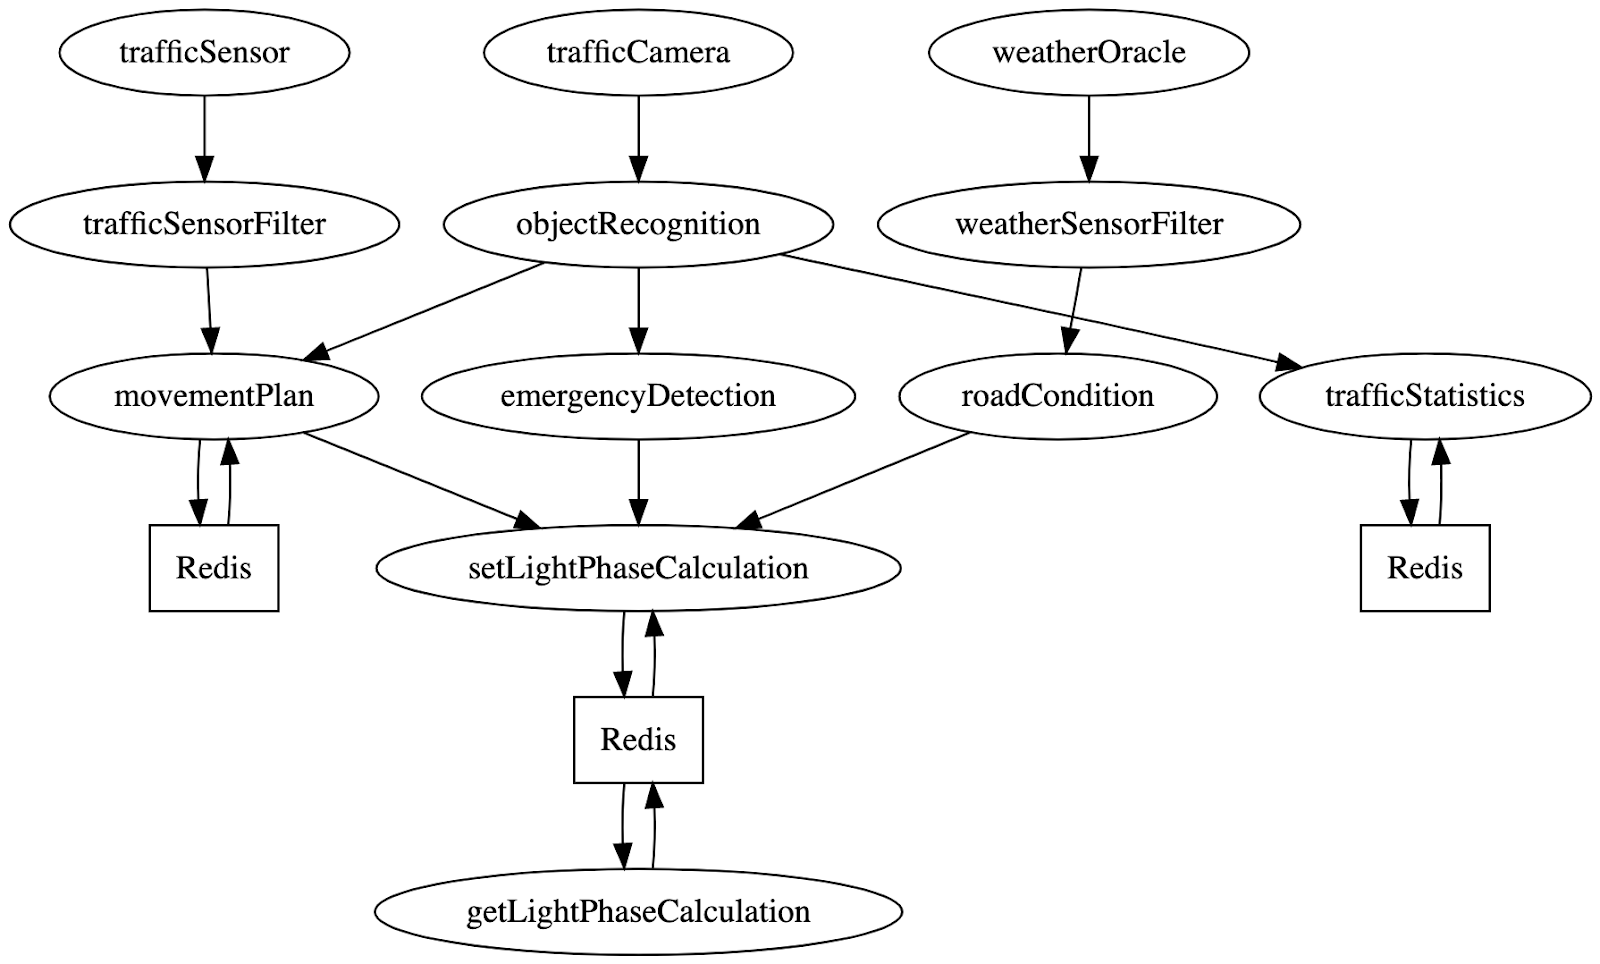
\includegraphics[width=\linewidth,keepaspectratio]{./iot-architecture-diagram.png}
\end{center}
\caption[IoT Architecture Diagram]{%
  Architecture diagram of our traffic light application.
  All functions communicate internally with each other via our library's RPC system
  and are thus automatically measured at runtime.
  The IoT devices in the top row (i.e.\@ trafficSensor, trafficCamera and weatherOracle) 
  represent the experiment's workload and are thus mocked in our setup (e.g.\@ by artillery workloads).%
}%
\label{fig:iotArchitectureDiagram}
\end{figure}

\begin{longtable}{l l} 
  \caption[IoT Function Overview]{IoT Function Overview\vspace*{1mm}}\label{tab:iotFunctionOverview}\\
  \textbf{Function} & \multicolumn{1}{c}{\textbf{Description}}\\ 
  \toprule
  %\endhead{}%
  trafficsensorfilter & \makecell[l]{Filters incoming traffic sensor data (e.g.\@ car speeds and directions), \\
    removing erroneous inputs.}\\
  \midrule[0.02em]
  objectrecognition & \makecell[l]{Analyses an uploaded camera image and detects different vehicles.}\\
  \midrule[0.02em]
  weathersensorfilter & \makecell[l]{Filters incoming weather sensor data, removing erroneous inputs.}\\
  \midrule[0.02em]
  movementplan & \makecell[l]{Uses database to aggregate found objects with their traffic attri- \\
    butes. Submits to setlightphasecalculation.}\\
  \midrule[0.02em]
  emergencydetection & \makecell[l]{Sends emergency status to setlightphasecalculation if respective \\
    objects were detected.}\\
  \midrule[0.02em]
  roadcondition & \makecell[l]{Evaluates (and scores) current road condition according to \\
    incoming weather data. Submits to setlightphasecalculation.}\\
  \midrule[0.02em]
  trafficstatistics & \makecell[l]{Saves seen objects to database for potential future analysis.}\\
  \midrule[0.02em]
  setlightphasecalculation & \makecell[l]{Aggragates all received input in database. Perpetually \\
    calculates light phases and updates traffic light in database. \\
    Responds to emergencies immediately (i.e.\@ without wait).}\\
  \midrule[0.02em]
  getlightphasecalculation & \makecell[l]{Returns current light phase.}\\
  \midrule[0.02em]
  \bottomrule
\end{longtable}

% TODO functionality description

% TODO Call Spec Appendix
Exact Function I/O specification can also be looked up within the source code\footnotemark.
There, each function has its own I/O behaviour (including individual examples) documented.
\footnotetext{\url{https://github.com/FaaSterMetrics/experiments/tree/master/experiments/iot/functions}}



\subsection{Benchmarking Properties}\label{ssec:webshopApplicationProperties}


\subsection{Specific Workloads}\label{ssec:webshopSpecificWorkloads}


\end{document}
